% !TeX root = documentation.tex
% !TeX spellcheck = de_DE

\section{Hintergründe}
Um die verschiedenen Eigenschaften anhand vom Lorenz-Modell erklären zu können, sind einige Hintergrundinformationen relevant. Diese davon sind im Folgenden beschrieben.

\subsection{Empfindlichkeit der Anfangsbedingungen}
Eine charakteristische Eigenschaft vom Lorenz-Attraktor ist, dass sehr kleine Unterschiede in den Anfangsbedingungen sehr grosse Unterschiede in der Lösungsmenge produzieren. Man nennt dies \textit{sensitive Abhängikeit} und das ist die wesentliche Komponente in chaotischen Systemen. 

So könnte zum Beispiel eine minimale Änderung am Startwert der Lorenz-Gleichungen die Lösung dazu bewirken, dass sie mit gleichbleibenden Parameter gerade auf der gegenüberliegenden Seite des Flügels im Plot zu liegen kommt. In Abbildung \ref{fig:lorenz-0} ist der Endpunkt gerade sehr nahe am Anfangspunkt (0.9 für x, y und z), wobei der Endpunkt in Abbildung \ref{fig:lorenz-1} auf dem anderen Flügel und durch die vielen anderen Werte überdeckt und deshalb nicht sichtbar ist. 

%TODO: Get on same line
\begin{figure}
\centering
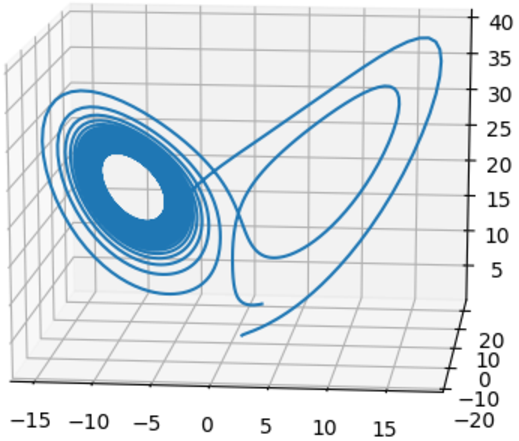
\includegraphics[width=0.5\linewidth]{lorenz/assets/lorenz-modell/lorenz09}
\caption{Bahn des Lorenz-Modell mit Startwert 0.9}
\label{fig:lorenz-0}
\end{figure}
\begin{figure}
\centering
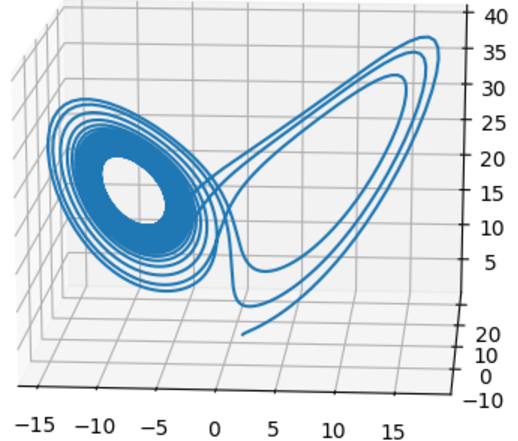
\includegraphics[width=0.5\linewidth]{lorenz/assets/lorenz-modell/lorenz10}
\caption{Bahn des Lorenz-Modell mit Startwert 1}
\label{fig:lorenz-1}
\end{figure}


Es gibt aber auch andere äussere Einwirkungen, die eine Veränderung der Werte auslösen kann. Zum Beispiel kann der Rundungsfehler eines CPUs die Ergebnisse klein wenig von Punkt-zu-Punkt verändern und so werden sich die Fehler kumulieren. Dies führt dazu, dass die Ergebnisse nicht reproduzierbar sind, da solche Einflüsse zwischen Durchläufen variieren.

\subsection{Chaostheorie}
Im Generellen ist die Chaostheorie ein Bereich der Mathematik der sich mit nicht-linearen dynamischen Systemen auseinandersetzt. Wie schon im vorherigen Abschnitt erwähnt ist die wesentliche Komponente eines chaotischen Systems die sensitive Abhängigkeit der Anfangsbedingungen. Sind beliebig kleine Unterschiede darin vorhanden, dann entwickelt sich das System nach einer endlichen Zeit völlig anders. Um das Verhalten eines chaotischen Systems zu einem bestimmten Zeitpunkt zu bestimmen, müssten für die Berechnung unendlich genaue Werte verwendet werden, was praktisch nicht möglich ist. Auch wenn chaotische Systeme deterministisch sind, ist es praktisch oftmals nicht möglich die Resultate an einem gesuchten Zeitpunkt genau zu bestimmen. 


Ein typisches Beispiel für ein chaotisches System ist das Wetter, wie Edward Lorenz herausgefunden hat. Die Modelle von Lorenz werden chaotisch genannt, weil sie auf den ersten Blick keinen Gesetzmässigkeiten folgen. Dennoch haben diese Systeme wiederkehrende Verhaltensweisen. Dies zeigt sich, indem sich wiederholende, zum Teil fraktale Muster und ähnliche Figuren zustande kommen. Durch das, dass die Parameter des Lorenz Modells aber mit heutiger Technik nicht unendlich genau gemessen werden kann, kann auch keine langfristige und verlässliche Aussage über das Wetter gemacht werden. 

\subsection{Attraktor}
In dynamischen Systemen ist ein Attraktor eine Untermenge eines Phasenraums(gewisse Anzahl an Zuständen), zu welchen sich ein dynamisches System im Laufe der Zeit zubewegt und diese Menge das System nicht mehr verlässt. \cite{wikiattraktor}
 Egal welche Startwerte man in einem Attraktor verwendet, das System entwickelt sich immer auf dieselbe Art und Weise. Im Bezug auf den Lorenz Attraktor ist dies die berühmte Form des Butterflys. Mathematisch formuliert ist ein Attraktor 


\begin{align}
\label{Attraktor} \text{Attraktor} &= \{ x_a,\varepsilon \in \mathbb{R}| \forall \varepsilon > 0 \nonumber\\
&\qquad {} \text{und} \nonumber\\
&\qquad {}  \forall T \exists t > T  \nonumber\\
&\qquad {}\text{gilt} \nonumber\\
&\qquad {} | x(t) - x_a | < \varepsilon \} 
\end{align}

Für jeden Zeitpunkt $T$ existiert ein späterer Zeitpunkt $t$, bei dem sich die Funktion $x$ (Lorenz-Attraktor) so entwickelt, dass der Betrag der Differenz kleiner als die Toleranz $\varepsilon$ wird. 

Als Beispiel könnte man, neben dem Lorenz-Attraktor, ein Pendel nehmen. Ein Pendel entwickelt sich mit der Zeit immer näher an einen Punkt, bei welchem sich alle darauf wirkenden Kräfte zu 0 addieren und sich das Pendel nicht mehr bewegt. Dieser Punkt ist also der Attraktor für dieses Pendelsystem. Im Unterschied zum Lorenz-Attraktor handelt es sich beim Pendelsystem aber um ein nicht-chaotisches System. Eine kleine Änderung in der Startposition der Masse am Ende des Pendels führt auf eine kleine Änderung in der Position, wobei es bei einem chaotischen System anders ausehen würde. 

\subsection{Strange Attraktor}
Beim Strange Attraktor wird ein normaler Attraktor um eine chaotische Komponenten erweitert. Das heisst, dass sich Werte innerhalb des Systems chaotisch verhalten. So könnten sich Lösungen in der Definition \eqref{Attraktor} innerhalb von $\varepsilon$ beliebig bewegen. Kleinste Parameter- oder Startpunktänderungen führen zu scheinbar zusammenhangslose Resultate. Dieses Verhalten wird wie in den vorherigen Abschnitten beschrieben Chaos genannt.
